\documentclass[UTF8]{ctexart} 
\usepackage{amsmath} % 提供数学符号支持
\usepackage{amssymb} % 提供更多数学符号支持
\usepackage{graphicx}% 用于插入图片
\usepackage[a6paper,centering,scale=0.8]{geometry} % 用于设置页面边距
\usepackage{float}%必须放到宏包的最后
\newenvironment{myquote}{\begin{quote}\kaishu\zihao{-5}}{\end{quote}}% 定义一个新的引用环境,使用楷体和小五号字体
\newtheorem{thm}{定理} % 定义定理环境,定理类环境thm
\newcommand\degree{^\circ}%定义新命令\degree(^\circ)

%可能存在依赖关系、功能覆盖或冲突
\begin{document}
\pagestyle{plain}
\title{\heiti杂谈勾股定理\thanks{省教育厅项目资助}}%标题,项目资助等,显示于文章首页下方
\pagestyle{plain}%为了使章节的页脚明确正确
\author{\kaishu 李汉龙 \thanks {沈阳建筑大学理学院}
\and \kaishu 隋英 \thanks {沈阳建筑大学理学院}
\and \kaishu 韩婷  \thanks{沈阳电视大学文法学院}}
\date{\today} % 日期,使用当前日期
\maketitle % 生成标题
\listoftables % 显示所有表格标签
\begin{abstract}
    这是一篇关于勾股定理的小短文。其中内容可能包含文字、公式、图形、表格等。
\end{abstract}
\tableofcontents % 生成目录
\section{勾股定理在古代}  
\label{sec:ancient}
西方称勾股定理为毕达哥拉斯定理,将勾股定理的发现归功于公元前6世纪
的毕达哥拉斯学派\cite{Kline}。该学派得到了一个法则,可以求出可排成直角
三角形三边的三元数组。毕达哥拉斯学派没有书面著作,该定理的严格表述和证明
则见于欧几里得\footnote{欧几里得,公元前 330-275年。}《几何原本》的命题 
47:“直角三角形斜边上的正方形等于两直角边上的两个正方形之和。”证明是用面积
做的。\par我国《周髀算经》载商高(约公元前12世纪)答周公问:
%\cite{Kline}引用参考文献Klin:\footnote{欧几里得,约公元前330-275年。}
%在页面下方加入脚注:欧几里得,约公元前300--275年;\par另起一行。
\begin{myquote}  
勾广三,股修四,径隅五。
\end{myquote}
又载陈子(公元前7--6世纪)答荣方向
\begin{myquote}
若求邪至日者,以日下为勾,日高为股,勾股各自乘,并而开方除之,得邪至日。
\end{myquote}  
都较古希腊更早,后者已经明确到处勾股定理的一般形式。图\ref{fig:xiantu}是我国古代对勾股定理的一种证明\cite{quanjing}  
%\red{fig:xiantu}用于读取标签\label{fig:xinatu},需要编译两次。
%\cite{quanjing}引用参考文献quanjing.
\begin{figure}[H]
\centering %开始插入图形,居中
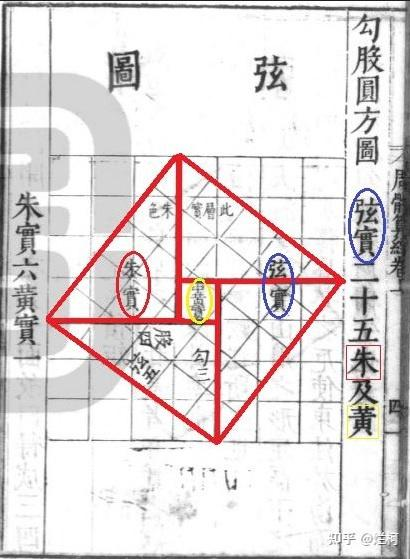
\includegraphics[scale=0.5]{images/xiantu.png}%插入图形,缩小0.5.
\caption{\zihao{-5}\kaishu宋赵爽在《周髀算经》中做的弦图(仿制),该图给出了勾股定理的一个极具对称美的证明。
\label{fig:xiantu}}%图形标题为楷书。
\end{figure}    %结束插入图形

勾股定理可以用现代语言装述如下·
\section{勾股定理的近代形式}%文章第二节,注意:每一节的标号自动按先后顺序生成。
\begin{thm}[勾股定理] 

直角三角形斜边的平方等于两腰的平方和。
\par 可以用符号语言表述为:设直角三角形 $ABC$,其中 $\angle C = 90^\circ$,则有
\begin{equation}
\label{eq:gougu} % 开始单行公式环境equation,其后加了书签gougu。
AB^2 = BC^2 + AC^2.
\end{equation} % 结束单行公式环境equation
\end{thm} % 结束定理环境。
 
满足式 \eqref{eq:gougu} 的整数称为\emph{勾股数}。第 \ref{sec:ancient} 节所说毕达哥拉斯学派得到的三元数组就是勾股数。下表列出一些较小的勾股数:\par
\eqref{eq:gougu} 读入书签 gougu;emph{勾股数},强调勾股数;\ref{sec:ancient} 读入书签 ancient;\par 另起一行。
 
\vspace{3mm} % 空一行。
 
\begin{tabular} {|c|c|c|}\hline % 开始表格环境,{|c|c|c|} 表示文字居中的三列,\hline...
% \hline 表示画两条并排的水平线。\hline 必须用于首行之前或者换行命令\\之后。
直角边 $a$ & 直角边 $b$ & 斜边 $c$ \\ \hline
3 & 4 & 5 \\ \hline
5 & 12 & 13 \\ \hline
\end{tabular} % 结束表格环境
 
($a^2 + b^2 = c^2$) % \$…\$ 表示数学环境,行内公式。
 
\begin{thebibliography}{99} % 参考文献开始。参考文献会自动编号,最大号码99。
\bibitem{1} 矢野健太郎. 几何的有名定理. 上海科学技术出版社, 1986. % 参考文献1。
\bibitem{quanjing} 曲安金. 商高、赵爽与刘徽关于勾股定理的证明. 数学传播, 20(3), 1998. % 参考文献2。
\bibitem{Kline} 克莱因. 古今数学思想. 上海科学技术出版社, 2002. % 参考文献3。
\end{thebibliography} % 参考文献结束。
 
\addcontentsline{toc}{section}{参考文献} % 在目录中添加“参考文献”的标记。
 
\begin{appendix} % 附录开始。
\section{附录} 勾股定理又叫商高定理,国外也称百牛定理。 % 附录内容。
\end{appendix} % 附录结束。
 
\end{document} % 文章结束,写在此后的所有内容都不起作用。







